% http://en.wikibooks.org/wiki/LaTeX/Title_Creation
% Adjusted for EPFL template


\begin{titlepage}

\begin{center}

%\raisebox{2cm}[-2cm][-2cm]{
%\hspace{-1.5cm}
%  \footnotesize
%  \begin{tabular}{@{\hspace{0pt}}l@{\hspace{0pt}} l@{\hspace{10pt}}}
%    \cline{1-1}     & \multirow{5}{*}{\hspace{10pt}\raisebox{-1ex}{\includegraphics[height=0.2\columnwidth]%%%{EPFL_LOG_QUADRI_Red}}}\\
%    EIDGEN\"{O}SSISCHE TECHNISCHE HOCHSCHULE LAUSANNE \\
%    POLITECNICO FEDERALE DI LOSANNA  \\
%    SWISS FEDERAL INSTITUTE OF TECHNOLOGY LAUSANNE  \\
%    \cline{1-1} \\
%    \raisebox{0.5ex}{\textbf{School of Computer and Communication Sciences}} \\
%    \raisebox{1.2ex}{Computer Science Section | Distributed Systems Laboratory (LSIR)} \\
%    
%  \end{tabular}
%}

%\raisebox{-1cm}[-2cm][-2cm]{
%\hspace{-1.5cm}
%
%  \footnotesize
%  \begin{tabular}{@{\hspace{0pt}}l@{\hspace{0pt}} l@{\hspace{10pt}}}
%    \cline{1-1}     & \multirow{5}{*}{\hspace{50pt}\raisebox{-1ex}{\includegraphics[height=0.2\columnwidth]{CERN-%logo.jpg}}}\\
%	ORGANISATION EUROP\'{E}EN POUR LA RECHERCHE NUCL\'{E}AIRE \\
%    \cline{1-1} \\
%    \raisebox{0.5ex}{\textbf{Information and Technology Department}} \\
%    \raisebox{1.2ex}{Digital Library Services} \\
%  \end{tabular}
%}


\raisebox{2cm}[1.5cm]{
\hspace{-2cm}
{\scriptsize
\begin{tabular} {|>{\centering\arraybackslash}m{8cm}>{\centering\arraybackslash}m{8cm}|}
\hline 
\hspace{0.1cm}

\raisebox{-1ex}{
\includegraphics[height=0.2\columnwidth]{EPFL_LOG_QUADRI_Red}} &
\raisebox{-1ex}{\includegraphics[height=0.2\columnwidth]{CERN-logo.jpg}}  \\ 
\multicolumn{2}{|c|}{ } \\ 
\multicolumn{2}{|c|}{ } \\  
\'{E}COLE POLYTECHNIQUE F\'{E}D\'{E}RALE DE LAUSANNE & ORGANISATION EUROP\'{E}EN POUR LA RECHERCHE NUCL\'{E}AIRE
\\
\multicolumn{1}{|l}{\textbf{School of Computer and Communication Sciences}} & 
\multicolumn{1}{l|}{\textbf{Information and Technology Department}} \\
\multicolumn{1}{|l}{Computer Science Section} & 
\multicolumn{1}{l|}{Digital Library Service} \\
\multicolumn{1}{|l}{Distributed Information System Laboratory (LSIR)} &  \\
\hline
\end{tabular}
}
}
\vspace{3\baselineskip}

\Large

\newcommand{\HRule}{\rule{\linewidth}{0.3mm}}


    {\LARGE \bfseries  $5e^{x+y}$: A Math Aware Search Engine (for CDS)} \\
	\vspace{3mm}    
    \textsc{\Large Master Thesis Project} \\
    
    %\HRule \\[0.2cm]
	
	\vspace{3mm}
	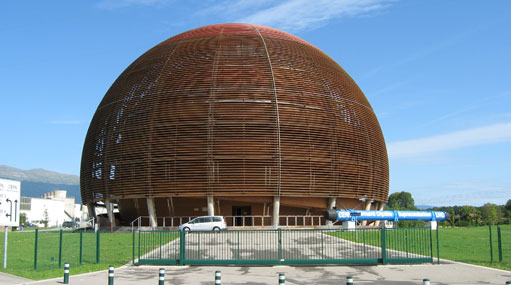
\includegraphics[height=6 cm]{cern_logo1.jpg}
	\vspace{3mm}
	\HRule 
	
	\emph{Author:} \\Arthur \textsc{Oviedo}\\
    \vspace{0.5cm}

    \emph{Supervisors:} \\   
    CERN: Nikolaos \textsc{Kasioumis} \\   
    EPFL: Karl \textsc{Aberer}\\
    
	\vspace{0.3cm}
    % Bottom of the page
    %\emph{March 2014}
	{\large \today}


\end{center}


\end{titlepage}

\newpage
\thispagestyle{empty}
\mbox{}